

\documentclass{sig-alternate-10pt}

\begin{document}

\title{SmartD: Smart Meter Data Analytics Dashboard}

\numberofauthors{1} 
\author{
% 1st. author
\alignauthor
Aylin Jarrah Nezhad, Tri Kurniawan Wijaya, Matteo Vasirani, Karl Aberer\\ 
       \affaddr{School of Computer and Communication Sciences}\\
       \affaddr{\a' ECOLE POLYTECHNIQUE F\a' ED\a' ERALE DE LAUSANNE EPFL}\\
       \affaddr{CH-1015 Lausanne, Switzerland}\\
       \email{firstname.lastname@epfl.ch}
\date{10 January 2014}
}
\maketitle

\begin{abstract}

Smart meters measure and communicate the real time energy consumption of  residential households to the utility companies. This data can be used for high quality data analysis which results in significant reduction of energy consumption. In this project we have implemented a web-based application to provide visualizations for comparison and prediction of customers behavior as energy consumers. This application visualizes the large dataset available from the Ireland smart metering project.

\end{abstract}


\section{Introduction} 

In the past the energy consumption data has been collected monthly or yearly just for billing purposes. The technological developments have recently made it possible to collect fine-grained data (e.g. hourly). This fine-grained data not only enables the billing according to dynamic pricing policies, but also leads to the development of new energy efficiency services. Aforementioned services are designed to guarantee the customer convenience and ensure improvement in economic activities.\\

Smart meters measure and communicate the real-time electricity consumption from residential households to the utility companies. The data collected from smart meters can be used for rich energy analysis such as customers consumption behavior analysis, theft detection, outage management, and conduct demand response events.\\

Several authors have done analytic studies on the energy consumption data. Some studies have looked at the possibilities of reduction in energy usage by providing the customers with feedback about their consumption behavior.\cite{1} While other studies have shown that it is possible to infer with high probability some households characteristics by analysis of the energy consumption.\cite{2,3}\\

The Irish Commission for Energy Regulation (CER) implemented The Smart Metering Electricity Customer Behavior Trials (CBTs) during 2009 and 2010. Over 5000 homes and businesses participated in this trial and had an electricity smart meter installed in their homes/premises. These smart meters had been sampling the electricity load measured in kWh every 30 minutes during this period. The information about the household characteristics was also collected through questionnaires. This information could relate to the presence and number of appliance in the house, household resident, his lifestyle, etc. This data has been made available for research purpose.\cite{4}\\

The data driven from smart meter trials can be used for comparison or prediction of customers behavior. For this purpose we need a data platform (e.g. application) that is able to retrieve required data with high velocity from a large dataset.\\
 
In our project, we have developed a web-based application that provides already mentioned functionalities. This application visualizes large volume of data published by CER, which contains over 20 million records for 782 customers. The web-interface is intuitive and simple to use. The visualization makes it easier for the users to \textbf{compare the energy consumption of individuals or groups of customers in different time slots}. \textbf{The distribution of energy consumption values for different customers in different time slots} enables the user to compare the amount of energy consumed by different households. Plotting the \textbf{predicted daily energy consumption for new customers} gives a clear idea about the customers behavior in future. As a result the energy consumption will decrease considerably by making the users aware of their behavior as electricity consumers.\\


\section{Visualizations}

In this project a web interface was developed over Global Sensor Networks (GSN). GSN is a software platform for processing the data streams generated by wireless sensor networks.\\
 
Virtual Sensors (VS) as the main component of GSN, receive the data from one or more wrappers. Wrappers are in charge of data acquisition for specific type of device.  Further Virtual Sensors process and store the data by using Virtual Sensor Processing classes (VSP).  Wrappers and VSPs are both written in java. A Virtual Sensor can be configured with an XML Virtual Sensor Description file (VSD). The selection and the parameterization of the VSP and Wrapper composing the VS will be contained in VSD file.\cite{5}\\
 
The SmartD project visualizes the energy consumption data. Any dataset of timestamped energy consumption values can be used for these visualizations (with little modifications). In this project the data published by CER was provided in a text file. This file should have been loaded into GSN database in order to be processed and visualized further. For this purpose we configured a new Virtual Sensor as an XML file. We employed CSV wrapper that generates GSN's stream elements by reading from text file. We also used a VSP called Bridge Virtual Sensor that receives the stream elements from CSV wrapper and inserts the data into GSN database. This process was taking 30 minutes to read 10000 records from the text file and insert them into database.  This result was not satisfactory, because of the large number of records (over 20 million) that we needed to load into database. In the end we had to import the data as sql files directly into GSN database without using any wrapper or VSP from GSN.\\ 


\subsection{Comparison of energy consumption for different customers}

We know that comparison of the energy consumption can provide a high quality data analysis. One of the most important factors that affect the amount of energy consumption is the time. The behavior of the customer as electricity consumer differs, depending on the time slot. For example if we consider the time slot as the time of the day, we can see the difference between the energy consumed during the night when most of the people are sleeping and in the evening when  most of the people are at home, watching TV, working on their laptops, etc. This difference can be also observed if we consider time slot as the season. Imagine hot summer days when air conditioners are working in most of the houses and offices 24 hours, and also beautiful spring days when nobody may need to turn the air conditioner on. As we can see the time affects not only the usage of electricity appliances but also the regularity of their use. Thus it affects the energy consumption pattern of the residential households.\\ 

In the current project we have implemented a web-based application that visualizes the energy consumption data for different individuals or groups of customers in different time slots. Figure 1 shows the interface provided for this visualization.\\

\begin{figure*}
\centering
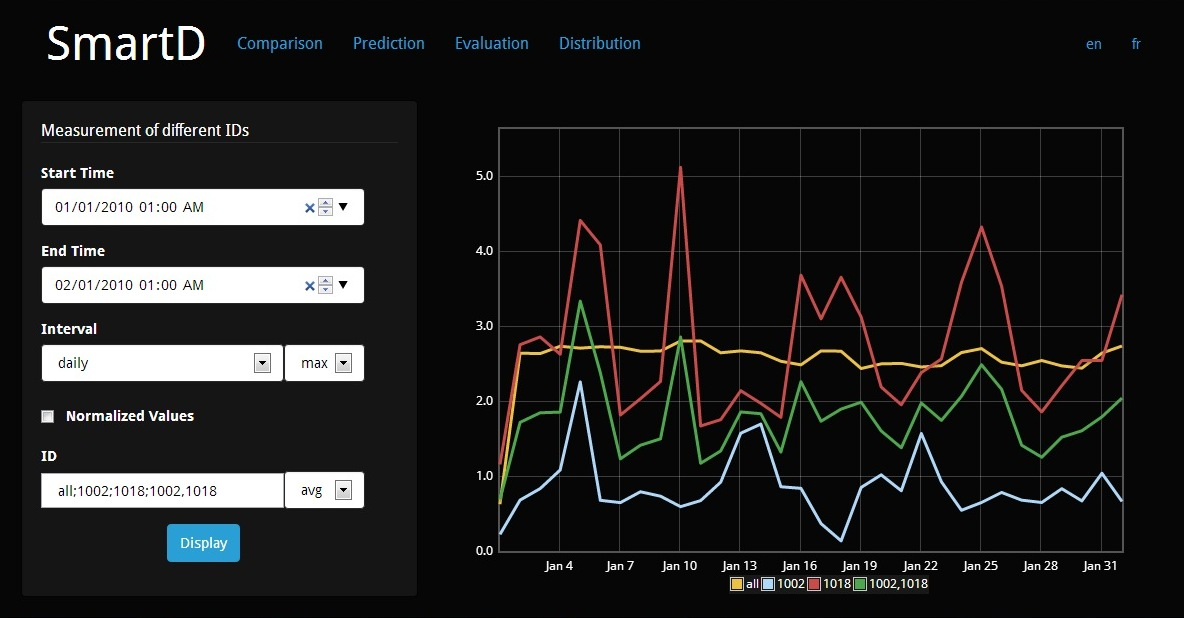
\epsfig{file=ComparisonFull.JPG, height=3in, width=6in}
\caption{Comparison of energy consumption for different meter IDs.}
\end{figure*}

\begin{figure}
\centering
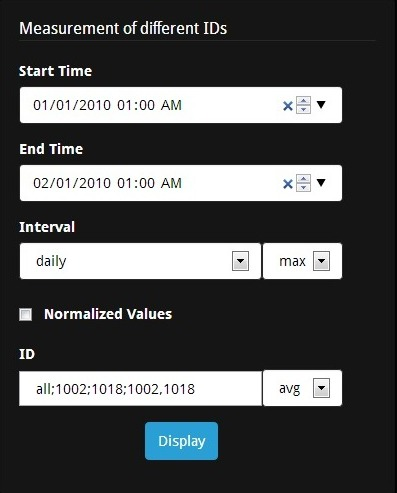
\epsfig{file=ComparisonControlPanel.JPG, height=3in, width=2in}
\caption{Control Panel for comparison of energy consumption for different customers.}
\end{figure}

The user can use the control panel shown in the Figure 2 to set the values such as start and end times, customer IDs, time interval, and normalization. The data will be retrieved and displayed on the plot based on the values set by the user.\\

\subsubsection{Time-interval selection} 

The data from Irish smart metering project is measured in the interval of 30 minutes. In this visualization the user can choose the time interval for which he wants to plot the data. The time interval can be set to every 30 minutes, hourly, daily, weekly or monthly. The user should also choose the kind of the aggregation (minimum, maximum, sum or average) that he wants to be used for the interval measurements. By setting this option the aggregated data will be plotted in the chosen time slot. In the Figure 3 the maximum of the data in the daily time interval has been chosen for each customer in the time slot from January first 2010, 01:00 AM to February first 2010, 01:00 AM.\\

\subsubsection{Customers selection}
  
In this visualization the user can also plot the data for all or groups of the customers. For this purpose the user should choose the groups containing the customer IDs and the kind of aggregation (minimum, maximum, sum or average) that he wants to be used for the data from each group of customers. The plot will display the aggregated energy consumption values for each group of customers as shown in the Figure 3. The groups of the customers should be separated by ";" and the customer IDs in each group should be separated by ",". The user can also use "all" as a group of all customers. This will enable the user to plot the aggregated data for all of the customers\footnote{In the Figure 1 the user has chosen "all;1002;1018;1002,1018" as the customer IDs. It means that the aggregated energy consumption will be displayed for following groups: 1) all of the customers 2) customer with ID=1002 3) customer with ID=1008 4) group of customers with IDs equal to 1002 and 1018.}.\\

Being able to visualize the data for all of the customers opens up some opportunities. For example it makes it easier to find the peak times in different time slots. It can also help to extract a general energy consumption pattern. This information can largely affect the development of new energy efficiency plans.\\  


\subsubsection{Normalization} 
This visualization also enables the user to plot the normalized values by setting the corresponding option in the control panel. The normalized value $Z$ can be calculated using the formula for standard score. For the value $x$ we will have: 
\begin{displaymath} Z = \frac{x - \mu}{\sigma} 
\end{displaymath}

where $\mu$ is the mean of the population, and $\sigma$ is the standard deviation of the population.\\

Figure 4 shows the maximum of the data in the daily time interval aggregated by average function and normalized for all of the customers, a group containing customers with IDs equal to 1002 and 1018, and the customers 1002 and 1018 individually plotted in the time slot from January first 2010 01:00 AM to February first 2010 01:00 AM. \\

\begin{figure}
\centering
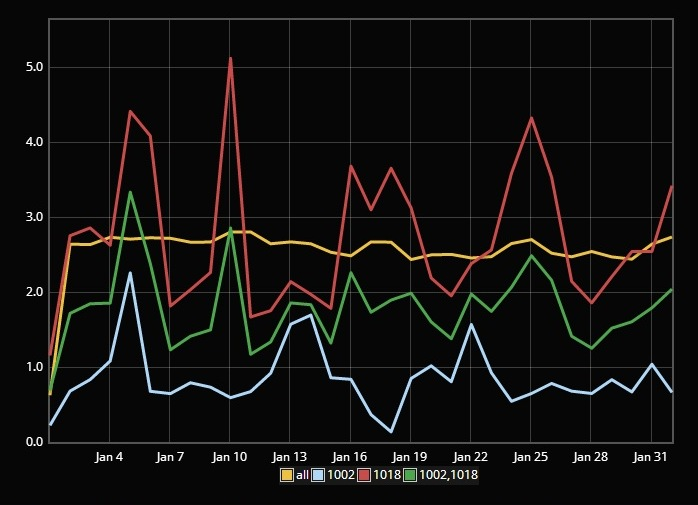
\epsfig{file=ComparisonPlot.JPG, height=2in, width=3in}
\caption{The maximum of the energy consumption in the daily time interval aggregated by average function for all of the customers, a group containing customers with IDs 1002 and 1018, and the customers 1002 and 1018 individually plotted in the time slot from January first 2010, 01:00 AM to February first 2010, 01:00 AM.}
\end{figure}

\begin{figure}
\centering
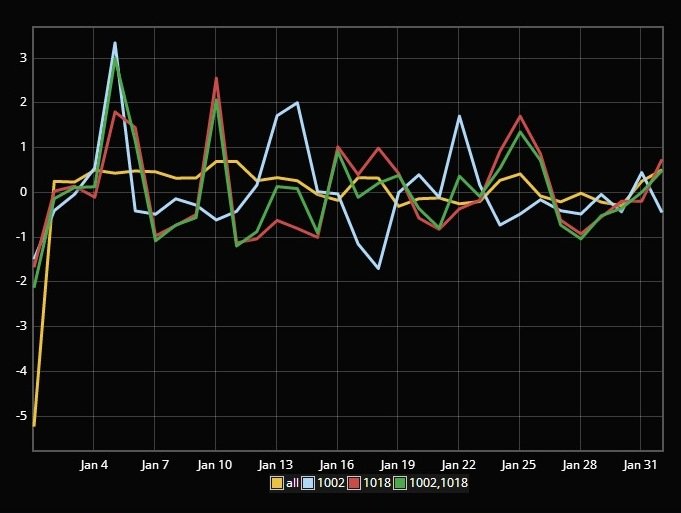
\epsfig{file=ComparisonPlotNormalized.JPG, height=2in, width=3.1in}
\caption{The maximum of the data in the daily time interval aggregated by average function and normalized for all of the customers, a group containing customers with IDs equal to 1002 and 1018, and the customers 1002 and 1018 individually plotted in the time slot from January first 2010 01:00 AM to February first 2010 01:00 AM.}
\end{figure}

All of these functionalities integrated in this visualization provide a platform that helps improving the comparison and data analysis.\\


\subsection{Prediction of customers' consumption behavior}

One of the important information that can be extracted from the available data is prediction of new customer's energy consumption behavior.\\
 
In the first section we considered time as one of the most important factors that can affect the amount of energy consumption. In this section we show that there are other factors such as household characteristics that play important role in increase or decrease of the amount of energy consumed by residential households.\\
 
In this project we aim to predict the new customers' energy consumption behavior. For this purpose we need to find the customers who are similar to the new customer the most and consider the average of their energy consumption per hour as the predicted energy consumption of that new customer. This will arise the question about how to find the similarity between the customers.\\ 

As it was mentioned before the Irish survey has provided valuable information about households characteristics. The participants (customers) have answered to 143 questions regarding their life style, age and number of residents, presence and number of electricity appliances, the characteristics of the house, etc. These household characteristics can help us to find the similarity between the customers.\\

We consider the questions about the characteristics of the households as features ($Q_1 \ldots Q_{143}$)\footnote {We should note that some questions should be taken as nominal features and some as numeric ones depending on the values that they can take as the answer. For example if the question is about the number of a special appliance in the house, the question will be numeric, since it can take an integer value as the answer. But if the question is about the presence of a special appliance in the house, the question will be nominal, since the answer can be "yes" or "no".} and the answers to the corresponding questions as the feature values ($A_1 \ldots A_{143}$), as shown in the Table 1. We find the euclidean distance between the customers based on their feature values (answers). The smaller the distance, the more the similarity between the customers.\\

In the next step we try to find the household characteristics associated with the amount of energy consumed. We consider the questions about the household characteristics as features. We assume that not all of the features (questions) are relevant to the amount of consumed energy. It means that there are some features that are redundant or irrelevant. The redundant features provide no more information than already selected features do and the irrelevant ones do not provide any useful information. There is an intelligent component that automatically selects the relevant features (questions). This component searches through all possible combination of the features to find which subset of the features works the best for the prediction of the energy consumption.\\

Table 2 shows how we find the relevant questions per hour. We consider questions as features ($Q_1 \ldots Q_{143}$) and energy consumption per hour as class label $h_i$ where $0 \le i \le 23$. For each customer we set the values ($A_1 \ldots A_{143}$) for the features. These values are the answers of the customer to the corresponding questions. The amount of consumed energy per hour can be found depending on the time context. In this project, the day of the week and the season provide us with the contextual information. We retrieve the average of daily energy consumption data for each customer per hour and based on the context. In the end we rank the questions by the frequency of their appearance as relevant features per hour.\\ 

The new customer should be asked to answer the highly ranked questions about their household characteristics. His answers can be used to find similar customers, and plot the average of their energy consumption data per hour as the new customer's predicted energy consumption behavior.\\

\begin{table}
\centering
\caption{Questions are features and Answers are feature values.}
\begin{tabular}{|c|c|l|} \hline
Customers&$Q_1 \ldots Q_{143}$\\ \hline
1 & $A_1 \ldots A_{143}$\\ \hline
$\vdots$ & $\vdots$\\ \hline
782 & $A_1 \ldots A_{143}$ \\ \hline
\end{tabular}
\end{table}

\begin{table}
\centering
\caption{Questions are features and Answers are feature values. Each hour of the day is class label and the average of energy consumption in that hour is its value.}
\begin{tabular}{|c|c|l|} \hline
Customers&$Q_1 \ldots Q_{143}$&Energy Consumption(EC) at $h_i$\\ \hline
1 & $A_1 \ldots A_{143}$ &EC of customer 1 at $h_i$\\ \hline
$\vdots$ & $\vdots$& $\vdots$\\ \hline
782 & $A_1 \ldots A_{143}$ &EC of customer 782 at $h_i$\\ \hline
\end{tabular}
\end{table}


There are two questions that should be addressed to provide a good estimation of the new customer energy consumption behavior :\\ \\

\begin{enumerate}
  \item What is the optimal number of highly ranked questions that should be asked in order to find similar customers?
  \item What is the optimal number of similar customers that should be considered for a better estimation of new customer's behavior?
\end{enumerate}
 
These two questions will be discussed in the next sub sections.\\


\subsubsection{Evaluation of similar customers' number}

In this section we show how to find the optimal number of similar customers that should be considered for a better estimation of the new customer energy consumption behavior.\\

The idea is to find the average of distances between the energy consumption of the customers and the energy consumption of their different number of nearest neighbors (most similar customers). The smallest distance provides the most similarity.\\ 
 
We consider the questions about the characteristics of the households as features ($Q_1 \ldots Q_{143}$) and the answers to the corresponding questions as the feature values ($A_1 \ldots A_{143}$), as shown in the Table 1. We find the euclidean distance between the customers based on their feature values (answers). The customers are most similar if the distance between them is the smallest.\\ 

For each customer we find the nearest neighbors and calculate the distances between the energy consumption of that customer and the energy consumption of different number of his nearest neighbors. In order to calculate the distances we consider the hours of the day to be the features and the average of energy consumption per hour to be the feature values as shown in the Table 3.\\

In Figure 5 we have fixed the number of highly ranked questions to 20 and have calculated the average of distances between the customers and their 1, 3, \ldots , 19 nearest neighbors. We need to find the number of nearest neighbors $n$ after which the average of distances does not decrease considerably.\\

Figure 5 displays the plot with the average of distances between the energy consumption of the customers and the energy consumption of their different number of nearest neighbors. We can see that for $n=9$ the decrease in average of distances falls bellow $\theta=0.5$. Thus 9 is the optimal number of similar customers to be considered.\\ 


\begin{table}
\centering
\caption{24 hours of the day are features and the averages of energy consumption per hour are the feature values.}
\begin{tabular}{|c|c|l|} \hline
Customers&Energy Consumption (EC)$h_0 \ldots h_{23}$\\ \hline
1 & EC of customer 1 $h_0 \ldots h_{23}$ \\ \hline
$\vdots$ & $\vdots$\\ \hline
782 & EC of customer 782 $h_0 \ldots h_{23}$\\ \hline
\end{tabular}
\end{table}

\begin{figure}
\centering
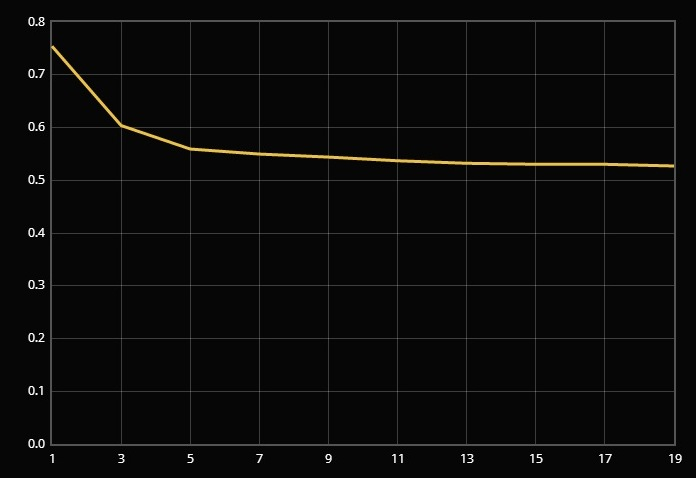
\epsfig{file=EvaluationNeighborNum.JPG, height=2in, width=3in}
\caption{Evaluation of similar customers' number. x-axis shows the number of nearest neighbors and the y-axis shows the average of distances between the energy consumption of the customers and the energy consumption of their nearest neighbors. We can see that the average of distances does not decrease substantially after 9.}
\end{figure}


\subsubsection{Evaluation of questions' number}

In this section we show how to find the optimal number of questions that should be considered in order to find similar customers.\\

We use the optimal number of similar customers obtained from the previous section. The idea is to find the distances between the energy consumption of the customers and their 9 nearest neighbors found by considering different number of highly ranked questions as features.\\

We consider the questions  as features and the answers to the corresponding questions as the feature values. We find the euclidean distance between the customers based on their answers to different number of highly ranked questions\footnote {For example first time we find the nearest neighbors by considering just one highly ranked question. Next time we find the nearest neighbors by considering three highly ranked question and so forth.}. The customers are most similar if the distance between them is the smallest.\\

For each customer we find 9 nearest neighbors and calculate the distances between the energy consumption of that customer and the energy consumption of his 9 nearest neighbors found for different number of highly ranked questions. In order to calculate the distances we consider the hours of the day to be the features and the average of energy consumption per hour to be the feature values as shown in the Table 3.\\ 

In Figure 6 we have calculate the average of distances between the customers and their 9 nearest neighbors for 1, 3, \ldots , 19 numbers of highly ranked questions. We need to find the number of questions $k$ after which the average of distances does not decrease considerably.\\

Figure 6 displays the plot with the average of distances between energy consumption of the customers and the energy consumption of their 9 number of nearest neighbors for different number of questions. We can see that for $k=5$ the decrease in average of distances falls bellow $\theta=0.4$. Thus 5 is the optimal number of questions to be asked for a better estimation of the new customer's energy consumption behavior.\\ 

\begin{figure}
\centering
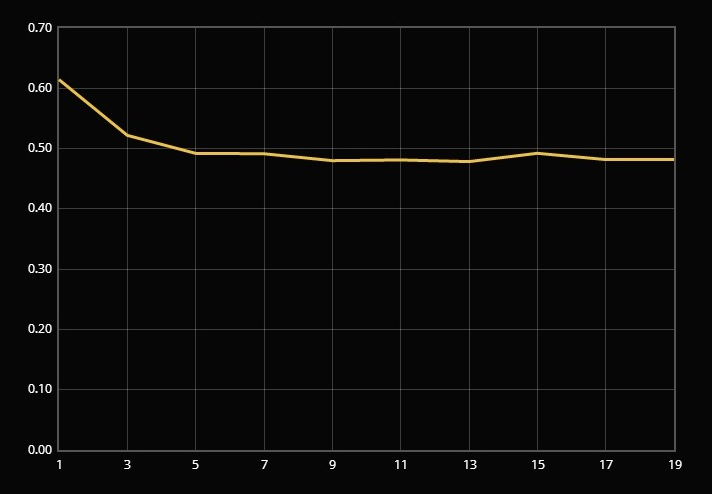
\epsfig{file=EvaluationQuestionNum.JPG, height=2in, width=3in}
\caption{Evaluation of questions' number. x-axis shows the number of the highly ranked questions and y-axis shows the average of distances between the energy consumption of the customers and the energy consumption of their 9 number of nearest neighbors. We can see that the average of distances does not decrease substantially after 5.}
\end{figure}

\subsubsection{Visualization}

This visualization displays a plot for new customers consumption behavior based on the contextual information and the behavior of similar customers.\\

As a result of the evaluations in previous sections the optimal number of similar customers is 7 and the optimal number of relevant questions is 5. It means that the new customer will be asked to answer to 5 relevant questions based on the context. Having the new customer's answers, we will be able to find 7 nearest neighbors and plot the average of their energy consumption per hour as the predicted energy consumption behavior of the new customer as shown in Figure 7.\\ 

The user sets the value for the season and the weekday (Sunday, \ldots , Saturday,  weekdays, weekend). The relevant questions will appear based on the provided context as shown in the Figure 9. The customer will be asked to answer to the relevant questions or to other questions from the list of all the questions shown in the Figure 8. When the user checks the checkbox for a question, that question will appear dynamically in the form shown in the Figure 9. The plot will display the predicted daily energy consumption of the new customer using the data from the new customer's 7 most similar customers. Figure 10 shows the plotted energy consumption behavior of the new customer.\\

For this visualization we have used the table containing all of the questions in our database. We had to make some changes to the questions' description to provide meaningful questions that could be suitable for our purposes. We also have created a new table that contains possible answers and their description for the closed questions. This table has 470 records that were added manually.\\


\begin{figure*}
\centering
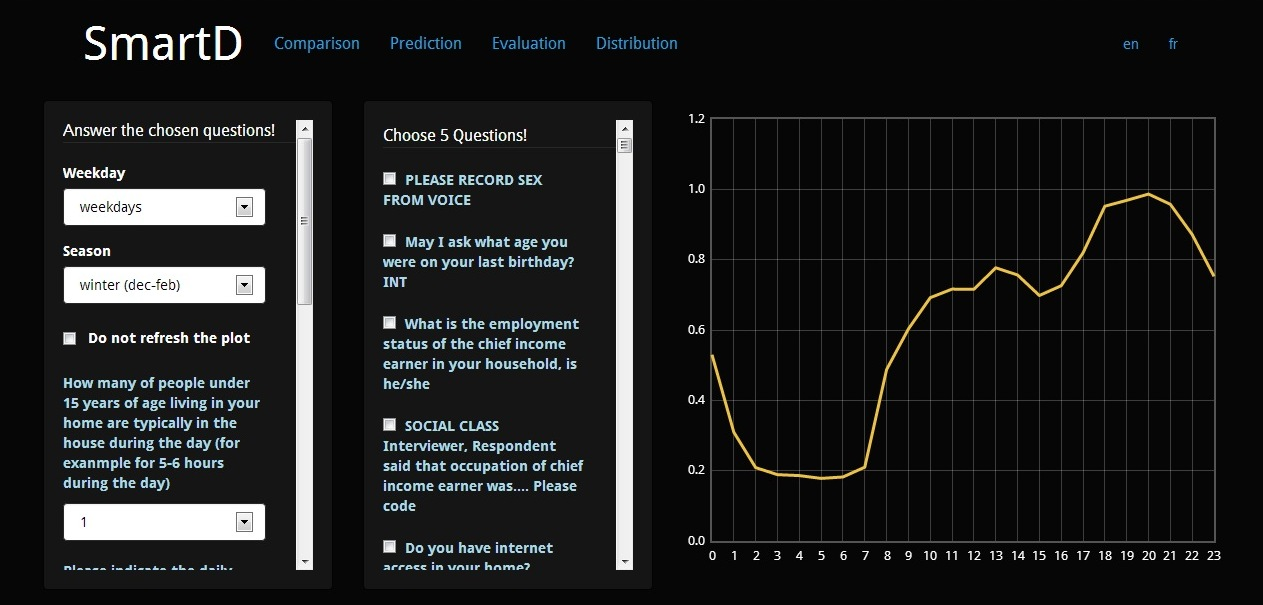
\epsfig{file=PredictionFull.JPG, height=2.7in, width=6in}
\caption{Prediction of customers' consumption behavior.}
\end{figure*}

\begin{figure}
\centering
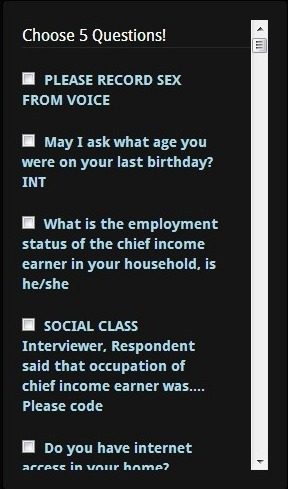
\epsfig{file=PredictionAllQuestions.JPG, height=3in, width=2in}
\caption{This form contains all of the questions. The user can check the check boxes in order to add the questions to the form containing the questions that the new customer should be asked.}
\end{figure}

\begin{figure}
\centering
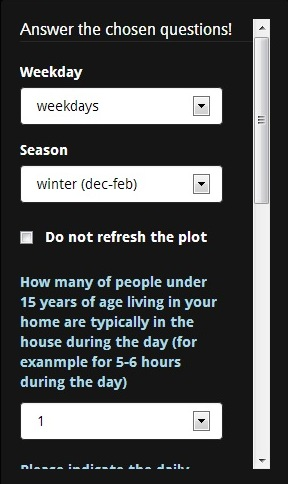
\epsfig{file=PredictionRelevantQuestions.JPG, height=3in, width=2in}
\caption{This form contains the contextual information and the questions that should be answered by the new customers.}
\end{figure}

\begin{figure}
\centering
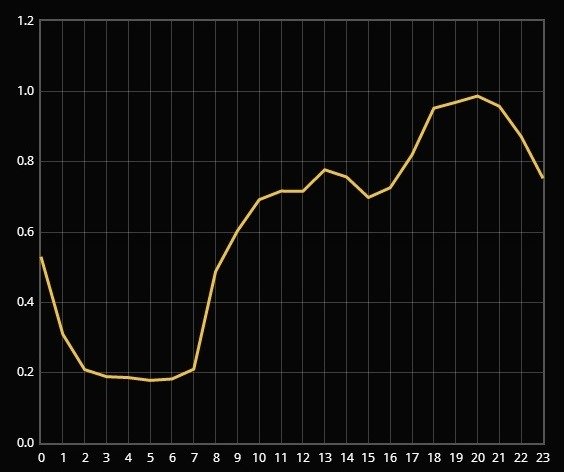
\epsfig{file=PredictionPlot.JPG, height=2.1in, width=3in}
\caption{This plot displays the predicted energy consumption behavior of the new customer per hour.}
\end{figure}

\subsection{Distribution of energy consumption for different customers in different time slots}

In this project we can retrieve the distribution of the energy consumption for different customers in different time slots and based on the bin size or number of the bins. For the visualization we can display the plot for the different bin sizes and different individual customers. In the case of number of the bins the visualizations can plot the distribution of the values just for one customer. The Figure 11 shows this visualization. The control panel shown in the Figure 12 can be employed in order to set the values such as start and end times, bin input and customer IDs. On the Figure 13 we can see the distribution of the energy consumption for the customers having the IDs 1002,1018 and 1014. 

\begin{figure*}
\centering
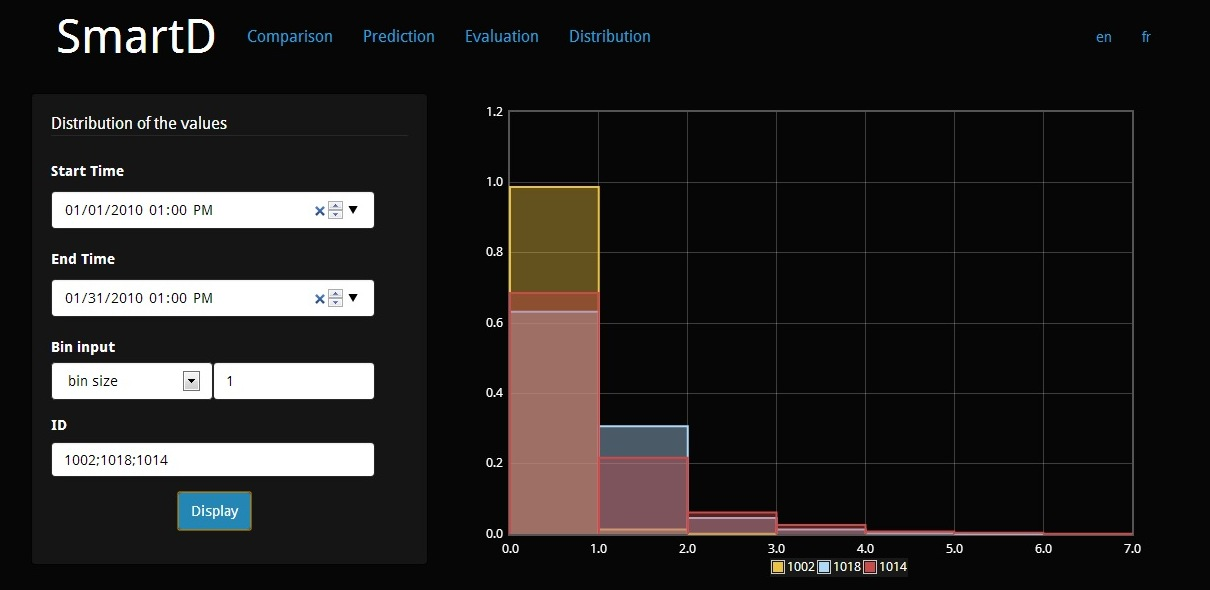
\epsfig{file=DistributionFull.JPG, height=3in, width=6in}
\caption{Distribution of values for different customers in different time slots.}
\end{figure*}


\begin{figure}
\centering
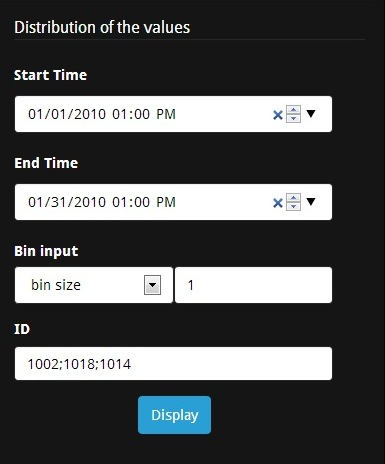
\epsfig{file=DistributionControlPanel.JPG, height=2.5in, width=2in}
\caption{Control Panel for distribution of the energy consumption for different customers.}
\end{figure}

\begin{figure}
\centering
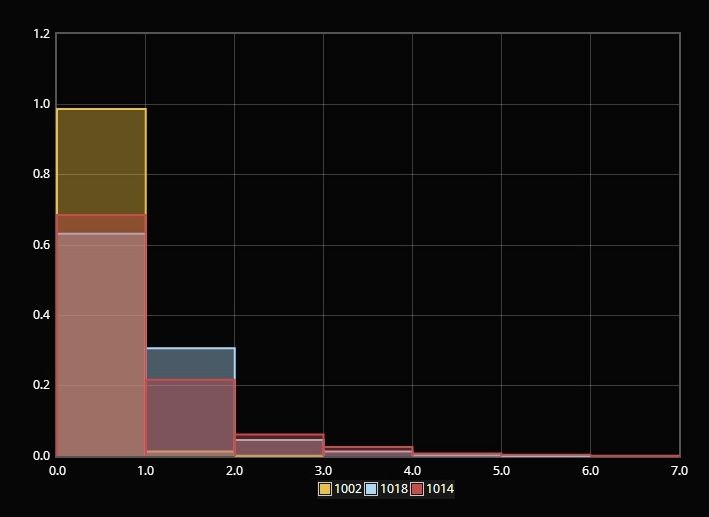
\epsfig{file=DistributionPlot.JPG, height=2.1in, width=3in}
\caption{Distribution of the energy consumption for different customers in different time slots.}
\end{figure}

\section{Implementation}

We have applied some open source libraries to implement this project.\\

The server side program is written in java. Java servlets are in charge of processing and preparing the data for the visualization. We have employed Weka's classes for the feature selection and calculation of distances (similarity) between the customers. Weka (Waikato Environment for Knowledge Analysis) is written in java and contains classes for data mining tasks such as clustering, classification, regression, visualization, and feature selection.\cite{6}\\

For the visualizations we have also used Javascript libraries such as jQuery and themes from Bootstrap.\cite{7,8}\\

\section{Future Work}

In the future work we can try to find energy saving plans. This can be done by clustering the customers based on their household characteristics to find out which characteristics result in less energy consumption. The most energy saving behavior can be suggested to the customers in order to reduce the amount of consumed energy and the billing costs. 

\section{Conclusions}

We have seen that we can extract valuable information by analyzing the energy consumption data. Several authors have done some studies on the energy consumption data. For example, some have used the energy consumption to classify the households and some other provided the consumer with personalized feedback, consumption visualization, automated control,etc, to see how these will affect the amount of energy consumed by the households.\\

In this work we have implemented a web-based platform that provides  functionalities needed in modern data analysis such as comparison and prediction of customers behavior by visualizing the large dataset available from the survey done in Ireland. These visualizations enable us to compare the energy consumption behaviors of different groups of customers in different time slots. Using the household characteristics, allow us to estimate the energy consumption of the new customers by considering the energy usage of the customers who were similar to them the most. We also have run evaluations to find the optimal number of nearest neighbors that should be considered and the optimal number of the highly ranked questions that should be asked to obtain a better estimation of the new customer's consumption behavior.\\



%\end{document}  % This is where a 'short' article might terminate


%
% The following two commands are all you need in the
% initial runs of your .tex file to
% produce the bibliography for the citations in your paper.
\bibliographystyle{abbrv}
\bibliography{sigproc}  % sigproc.bib is the name of the Bibliography in this case
% You must have a proper ".bib" file
%  and remember to run:
% latex bibtex latex latex
% to resolve all references
%
% ACM needs 'a single self-contained file'!
%
%APPENDICES are optional
%\balancecolumns

\begin{thebibliography}{10}

\bibitem{1}
J. Stragier, L. Hauttekeete, L. De Marez, "Reducing Household' Energy Use: A Segmentation of Flanders on Adoption Intention of Smart Metering Technology," World Renewable Energy Congress 2011.
\bibitem{2}
C. Beckel, L. Sadamori, and S. Santini, "Automatic Socio-Economic Classification of Households Using Electricity Consumption Data,"ACM, 2013.
\bibitem{3}
F. Fusco, M. Wurst, J. W. Yoon, "Mining Residential Household Information from Low-resolution Smart Meter Data,"21st International Conference on Pattern Recognition (ICPR 2012).
\bibitem{4}
Commission for Energy Regulation. Smart Metering Trial Data Publication, 2012.
\bibitem{5}
GSN Team, "Global Sensors Networks", July 2, 2009.
\bibitem{6}
http://weka.wikispaces.com/
\bibitem{7}
http://getbootstrap.com/
\bibitem{8}
http://jquery.com/

\end{thebibliography}

%\appendix
%%Appendix A
%\section{Headings in Appendices}
%
%
%
%
%\subsection{Introduction}
%\subsection{The Body of the Paper}
%\subsubsection{Type Changes and  Special Characters}
%\subsubsection{Math Equations}
%\paragraph{Inline (In-text) Equations}
%\paragraph{Display Equations}
%\subsubsection{Citations}
%\subsubsection{Tables}
%\subsubsection{Figures}
%\subsubsection{Theorem-like Constructs}
%\subsubsection*{A Caveat for the \TeX\ Expert}
%\subsection{Conclusions}
%\subsection{Acknowledgments}
%\subsection{Additional Authors}
%
%
%\subsection{References}

% This next section command marks the start of
% Appendix B, and does not continue the present hierarchy

\end{document}
